\chapter{Especificação de Requisitos} \label{cap:especificacao}

A análise comparativa das arquiteturas apresentadas no Capítulo 3 evidenciou que nenhuma das propostas indiviuldamente atende de forma plena ao conjunto de objetivos do sistema. A arquiteuira com BOLO (Seção 3.1) preserva a operacionalidade em tempo real, mas não formaliza mecanismos criptográficos robustos para o acesso investigativo retrospectivo. A Arquitetura de Vigilância Criptografada com Governança por Quórum (Seção 3.2) introduz camadas bem definidas de custódia e governança, porém não integra o fluxo BOLO ao modelo criptográfico. Por fim, a Arquiteura com Threshold Criptográfico (Seção 3.3), embora a mais completa do ponto de vista da governança distribuída, apresenta uma vulnerabilidade estrutural no momento de reconstrução da chave mestra: ao exigir que os fragmentos sejam reunidos no ambiente computacional do solicitante, a chave torna-se temporariamente exposta, comprometendo a integridade do sistema e exigindo um reset e redistribuição dos fragmentos após cada ativação do fluxo de emergência.

A Arquitetura 3.0, cujo diagrama está reproduzido na Figura 4, representa a síntese dessas três propostas e constitui a arquitetura selecionada para implementação. Ela incorpora o fluxo BOLO integrado ao ciclo de vida do dado criptografado, mantém as camadas de borda, custódia, governança e acesso da proposta anterior, e resolve a vulnerabilidade de exposição da chave ao adotar chaves mensais independentes — geradas como pares assimétricos (PK, SK) — cujos fragmentos são distribuídos ao Comitê de Emergência via Shamir's Secret Sharing. Com isso, a reconstrução da chave para acesso excepcional fica circunscrita ao mês de interesse, impedindo que uma ativação do fluxo de emergência comprometa registros de outros períodos. Adicionalmente, a arquitetura formaliza três modalidades distintas de busca (Aberta, Fechada e Total), cada uma com escopo, custo computacional e requisitos de autorização próprios.

\begin{figure}[H]
    \centering
    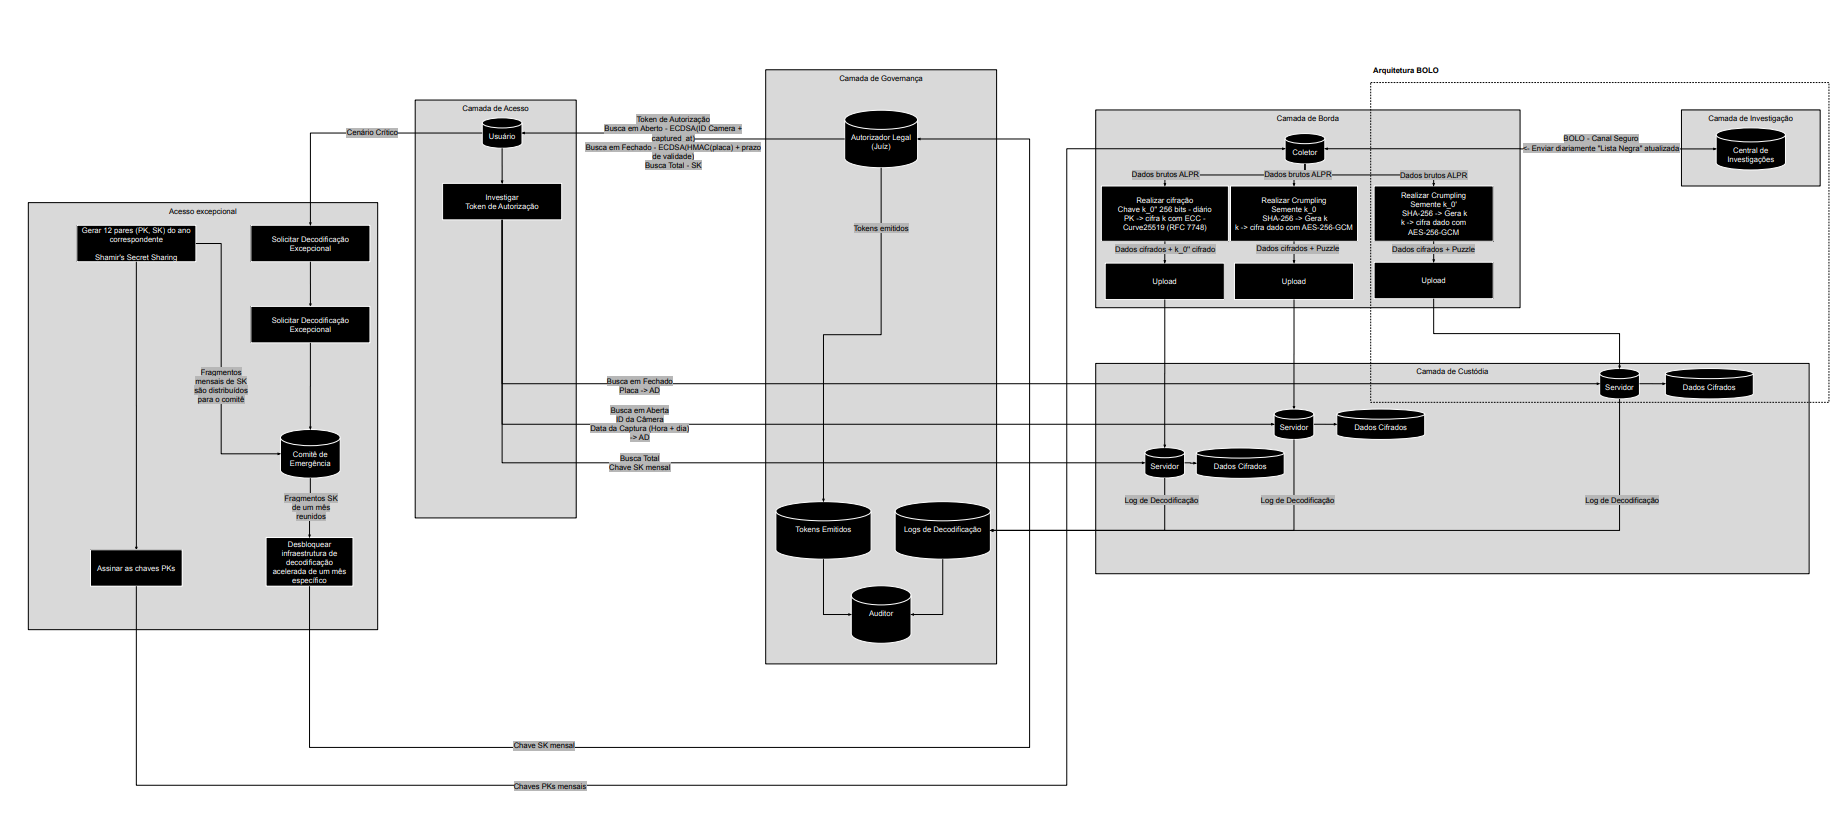
\includegraphics[width=1.0\textwidth]{Imagens/Cap4/arquitetura.png}
    \caption{Fluxograma da Arquitetura do Sistema}
    \label{fig:arquitetura-bolo-quorum}
\end{figure}

\section{Modalidades de Busca}
A Busca em Aberto é orientada por metadados não identificadores e destina-se à localização de eventos por câmera e por janela temporal. Nessa modalidade, o token de autorização é assinado com ECDSA sobre a combinação entre o identificador da câmera e o instante de captura (\textit{ECDSA}($ID_{camera} + captured\_at$)). Como não há exposição direta da identidade do veículo, essa forma de consulta é adequada para auditorias de fluxo e verificações operacionais.

A Busca em Fechado visa um veículo específico e exige que o token de autorização vincule o HMAC da placa a um prazo de validade explícito (\textit {ECDSA}($HMAC_{placa} + prazo\_de\_validade$)). O prazo limita temporalmente o escopo da autorização, impedindo que uma ordem judicial seja reutilizada indefinidamente.

A Busca Total destina-se exclusivamente a cenários de acesso excepcional mediados pelo Comitê de Emergência. Nela, a chave secreta mensal (SK) é reconstruída a partir do quórum de fragmentos via Shamir's Secret Sharing e empregada para decifrar o conjunto de registros do período. Cada ativação deste fluxo gera um log de decodificação auditável e é restrita ao mês cujos fragmentos foram reunidos, sem comprometer chaves de outros períodos. Esta separação resolve diretamente a vulnerabilidade identificada na Seção 3.3: ao segmentar as chaves em granularidade mensal, uma ativação do fluxo de emergência não concede acesso retroativo ou prospectivo irrestrito — o impacto de cada ativação fica circunscrito ao mês específico, e o conjunto de fragmentos não necessita de reset global após cada uso.

\section{Requisitos Funcionais}
\noindent\textbf{RF01 — Crumpling na borda:} O coletor ALPR deve, para cada captura, gerar uma semente aleatória $k_0$ de 256 bits, derivar a chave de cifragem k via SHA-256, cifrar o payload com AES-256-GCM e descartar imediatamente o texto claro da placa e a semente $k_0$ após o upload.

\noindent\textbf{RF02 — Puzzle criptográfico:} O sistema deve gerar, junto a cada registro cifrado, um puzzle de prova de trabalho com entropia configurável pelo Conselho de Governança, de modo que a resolução do puzzle seja condição necessária para a decodificação de qualquer registro.

\noindent\textbf{RF03 — Fluxo BOLO:} O sistema deve suportar a consulta em tempo quase real de placas capturadas contra uma lista negra atualizada diariamente pela Central de Investigações via canal seguro, sem que essa verificação exija a decodificação do registro armazenado no servidor.

\noindent\textbf{RF04 — Gestão de chaves mensais:} O sistema deve gerar anualmente 12 pares de chaves assimétricas mensais (PK, SK) baseadas em criptografia de curva elíptica Curve25519 (RFC 7748), assinar as chaves públicas e distribuir os fragmentos das chaves secretas ao Comitê de Emergência via Shamir's Secret Sharing antes do início de cada mês.

\noindent\textbf{RF05 — Cifragem com chave pública mensal:} Na modalidade de Busca Total, o coletor deve cifrar a chave de sessão diária $k_0''$ com a chave pública mensal (PK) via ECC-Curve25519, armazenando o dado cifrado e a chave de sessão cifrada no servidor.

\noindent\textbf{RF06 — Emissão e verificação de tokens de autorização:} O sistema deve suportar a emissão de tokens de autorização assinados digitalmente pelo Autorizador Legal (Judiciário) e verificar sua assinatura e escopo antes de liberar qualquer operação de decodificação.

\noindent\textbf{RF07 — Modalidades de busca diferenciadas:} O sistema deve implementar as três modalidades de busca descritas na Seção 4.1, garantindo que cada modalidade exija o tipo de token correspondente e imponha o custo computacional adequado ao seu escopo.

\noindent\textbf{RF08 — Log de decodificação:} Toda operação de decodificação deve gerar um registro imutável de auditoria contendo ao menos: identificador do token utilizado, timestamp da operação, modalidade de busca e identificador do operador.

\noindent\textbf{RF09 — Reconciliação de auditoria:} O Auditor deve ter acesso a uma interface de reconciliação que permita cruzar os tokens emitidos pelo Autorizador Legal com os logs de decodificação gerados pelo servidor, sinalizando automaticamente qualquer discrepância entre o volume autorizado e o volume efetivamente decodificado.

\noindent\textbf{RF10 — Acesso excepcional por quórum:} O sistema deve implementar o fluxo de Busca Total de modo que a reconstrução da chave SK mensal exija um quórum mínimo configurável de membros do Comitê de Emergência, e que a decodificação seja restrita ao mês cujos fragmentos foram reunidos.

\section{Requisitos Não-Funcionais}
\noindent\textbf{RNF01 — Independência de chaves:} A resolução de um puzzle ou a decodificação de um registro não deve reduzir o custo computacional para decodificação de nenhum outro registro, garantindo que o custo de vigilância em massa escale linearmente com o volume de dados acessados.

\noindent\textbf{RNF02 — Confidencialidade na borda:} O texto claro da placa não deve persistir em nenhum componente de borda após a cifragem e o upload do registro, eliminando a possibilidade de extração de PII a partir dos coletores.

\noindent\textbf{RNF03 — Rastreabilidade perene:} Toda operação de acesso, desde a emissão do token até a conclusão da decodificação, deve ser registrada de forma auditável e imutável, de modo que o volume de decodificações realizadas por um usuário seja verificável retroativamente pelo Conselho de Governança.

\noindent\textbf{RNF04 — Isolamento temporal de chaves de emergência:} A ativação do fluxo de Busca Total para um determinado mês não deve comprometer a confidencialidade dos registros de outros meses. Este requisito é garantido pela segmentação das chaves SK em granularidade mensal, resolvendo a vulnerabilidade identificada na Seção 3.3.

\noindent\textbf{RNF05 — Proporcionalidade de custo:} O parâmetro de entropia dos puzzles deve ser calibrado pelo Conselho de Governança de forma que o custo de decodificação de um único veículo seja operacionalmente viável para investigações legítimas, enquanto o custo acumulado de varreduras massivas seja orçamentariamente proibitivo para qualquer entidade com orçamento público finito.

\noindent\textbf{RNF06 — Integridade dos registros:} O uso de Associated Data (AD) no esquema AES-256-GCM deve garantir que qualquer adulteração no ciphertext ou nos metadados de câmera invalide a decifragem, protegendo a cadeia de custódia das evidências.

\noindent\textbf{RNF07 — Disponibilidade do fluxo BOLO:} O subsistema de consulta BOLO deve operar de forma independente do servidor de dados históricos, de modo que indisponibilidades na camada de custódia não interrompam alertas operacionais em tempo real.

\noindent\textbf{RNF08 — Auditabilidade do Comitê de Emergência:} Toda ativação do fluxo de Busca Total deve gerar rastros administrativos públicos e auditáveis, tornando qualquer tentativa de vigilância em larga escala institucionalmente visível e politicamente rastreável.
